\section{Задание}
По выданному преподавателем варианту восстановить текст заданного варианта программы, определить предназначение и составить описание программы, определить область представления и область допустимых значений исходных данных и результата, выполнить трассировку программы.
\begin{figure}[H]
\centering
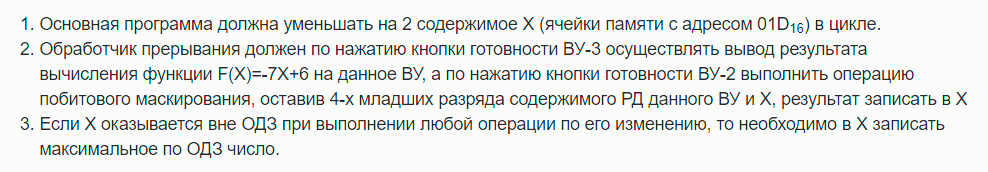
\includegraphics[scale=0.6]{task}
\label{pic:task}
\end{figure}

\section{Текст программы}
\begin{center}
\begin{tabular}{|c|c|c|l|}
\hline
\textbf{Адрес ячейки} & \textbf{Содержимое ячейки} & \textbf{Мнемоника} & \textbf{Комментарии}\\
\hline
5BA & 05CD & --- & Адрес начала массива\\
5BB & A000 & --- & Ячейка для хранения адреса\\
		   & & & обрабатываемого элемента массива\\
5BC & E000 & --- & Ячейка для хранения количества\\
		   & & & необработанных элементов массива\\
5BD & E000 & --- & Неиспользуемая обнуляемая ячейка\\
\hline
5BE & 0200 & CLA & Загружаем ноль в ячейку 5BD\\
5BF & EEFD & ST IP$-$3 & (далее не используется)\\
5C0 & AF05 & LD \#5 & Помещаем количество элементов\\
5C1 & EEFA & ST IP$-$6 & массива в ячейку 5BC\\
5C2 & 4EF7 & ADD IP$-$9 & Помещаем адрес элемента, следующего\\
5C3 & EEF7 & ST IP$-$9 & за последним, в ячейку 5BB\\
5C4 & ABF6 & LD $-$(IP$-$10) & Уменьшаем ячейку 5BB на 1 и\\
5C5 & 0480 & ROR & загружаем следующий элемент массива\\
5C6 & 0380 & CMC & Если элемент четный, то\\
5C7 & F402 & BCS IP$+$2 & выставляем C=1\\
5C8 & 0380 & CMC & Если элемент нечетный,\\
5C9 & 0400 & ROL & оставляем исходное состояние C\\
5CA & 85BC & LOOP 0x5BC & Если остались необработанные\\
5CB & CEF8 & JMP IP$-$8 & элементы, переходим к адресу 5С4\\
5CC & 0100 & HLT & Если нет, завершаем программу\\
\hline
5CD & 0480 & --- &\\
5CE & 0601 & --- &\\
5CF & F000 & --- & Элементы массива\\
5D0 & 0900 & --- &\\
5D1 & 0A00 & --- &\\
\hline
\end{tabular}
\end{center}

\newpage

\section{Описание программы}
\subsection{Назначение программы}
Программа проходит каждый элемент массива с конца и исследует его элементы на четность (признак четности --- последний бит элемента). Если элемент является четным, то программа устанавливает флаг `C' , в противоположенном же случае сохраняет исходное состояние флага. Элементы массива в ходе исполнения программы не изменяются. Ячейка над первой командой программы обнуляется. Результат работы программы невозможно представить в виде функции.

\subsection{Область представления и область допустимых значений данных}
\noindent Ячейки 5CD--5D1 (элементы массива): 16-разрядные без-/знаковые целые числа, $-2^{15}\ldots2^{15}-1$/$0\ldots2^{16}-1$\\
Ячейка 5BA (адрес начала массива): 11-разрядное беззнаковое целое число, $0\ldots2^{11}-1$\\
Ячейки 5BB--5BD: любые допустимые в рамках БЭВМ значения

\subsection{Расположение в памяти ЭВМ}
\noindent Расположение программы: 5BE--5CC\\
Ячейка для хранения адреса начала массива: 5BA\\
Элементы массива: (5BA)--(5BA)$+5$\\
Обнуляемкая ячейка: 5BD\\
Вспомогательные ячейки, заполняющиеся по ходу работы программы: 5BB--5BC

\subsection{Адреса первой и последней выполняемой команд программы}
\noindent Адрес первой команды программы: 5BE\\
Адрес последней команды программы: 5СС

\section{Таблица трассировки}
\begin{center}
\begin{tabular}{|c|c|c|c|c|c|c|c|c|c|c|c|}
\hline
\multicolumn{2}{|c}{\makecell{\textbf{Выполняемая}\\\textbf{команда}}}
  &\multicolumn{8}{|c|}{\textbf{Содердимое регистров после выполнения команды}}
  &\multicolumn{2}{c|}{\makecell{\textbf{Ячейка, содержимое}\\\textbf{которой изменилось}}}\\
\hline
Адрес & Код & IP & CR & AR & DR & SP & BR & AC & NZVC & Адрес & Новый код\\
\hline
5BE & 0200 & 5BF & 0200 & 5BE & 0200 & 000 & 05BE & 0000 & 0100 & --- & ---\\
\hline
5BF & EEFD & 5C0 & EEFD & 5BD & 0000 & 000 & FFFD & 0000 & 0100 & 5BD & 0000\\
\hline
5C0 & AF05 & 5C1 & AF05 & 5C0 & 0005 & 000 & 0005 & 0005 & 0000 & --- & ---\\
\hline
5C1 & EEFA & 5C2 & EEFA & 5BC & 0005 & 000 & FFFA & 0005 & 0000 & 5BC & 0005\\
\hline
5C2 & 4EF7 & 5C3 & 4EF7 & 5BA & 05CD & 000 & FFF7 & 05D2 & 0000 & --- & ---\\
\hline
5C3 & EEF7 & 5C4 & EEF7 & 5BB & 05D2 & 000 & FFF7 & 05D2 & 0000 & 5BB & 05D2\\
\hline
5C4 & ABF6 & 5C5 & ABF6 & 5D1 & 0A00 & 000 & FFF6 & 0A00 & 0000 & 5BB & 05D1\\
\hline
5C5 & 0480 & 5C6 & 0480 & 5C5 & 0480 & 000 & 05C5 & 0500 & 0000 & --- & ---\\
\hline
5C6 & 0380 & 5C7 & 0380 & 5C6 & 0380 & 000 & 05C6 & 0500 & 0001 & --- & ---\\
\hline
5C7 & F402 & 5CA & F402 & 5C7 & F402 & 000 & 0002 & 0500 & 0001 & --- & ---\\
\hline
5CA & 85BC & 5CB & 85BC & 5BC & 0003 & 000 & 05CA & 0500 & 0001 & 5BC & 0004\\
\hline
5CB & CEF8 & 5C4 & CEF8 & 5CB & 05C4 & 000 & FFF8 & 0500 & 0001 & --- & ---\\
\hline
5C4 & ABF6 & 5C5 & ABF6 & 5D0 & 0900 & 000 & FFF6 & 0900 & 0001 & 5BB & 05D0\\
\hline
5C5 & 0480 & 5C6 & 0480 & 5C5 & 0480 & 000 & 05C5 & 8480 & 1010 & --- & ---\\
\hline
5C6 & 0380 & 5C7 & 0380 & 5C6 & 0380 & 000 & 05C6 & 8480 & 1011 & --- & ---\\
\hline
5C7 & F402 & 5CA & F402 & 5C7 & F402 & 000 & 0002 & 8480 & 1011 & --- & ---\\
\hline
5CA & 85BC & 5CB & 85BC & 5BC & 0002 & 000 & 05CA & 8480 & 1011 & 5BC & 0003\\
\hline
5CB & CEF8 & 5C4 & CEF8 & 5CB & 05C4 & 000 & FFF8 & 8480 & 1011 & --- & ---\\
\hline
5C4 & ABF6 & 5C5 & ABF6 & 5CF & F000 & 000 & FFF6 & F000 & 1001 & 5BB & 05CF\\
\hline
5C5 & 0480 & 5C6 & 0480 & 5C5 & 0480 & 000 & 05C5 & F800 & 1010 & --- & ---\\
\hline
5C6 & 0380 & 5C7 & 0380 & 5C6 & 0380 & 000 & 05C6 & F800 & 1011 & --- & ---\\
\hline
5C7 & F402 & 5CA & F402 & 5C7 & F402 & 000 & 0002 & F800 & 1011 & --- & ---\\
\hline
5CA & 85BC & 5CB & 85BC & 5BC & 0001 & 000 & 05CA & F800 & 1011 & 5BC & 0002\\
\hline
5CB & CEF8 & 5C4 & CEF8 & 5CB & 05C4 & 000 & FFF8 & F800 & 1011 & --- & ---\\
\hline
5C4 & ABF6 & 5C5 & ABF6 & 5CE & 0601 & 000 & FFF6 & 0601 & 0001 & 5BB & 05CE\\
\hline
5C5 & 0480 & 5C6 & 0480 & 5C5 & 0480 & 000 & 05C5 & 8300 & 1001 & --- & ---\\
\hline
5C6 & 0380 & 5C7 & 0380 & 5C6 & 0380 & 000 & 05C6 & 8300 & 1000 & --- & ---\\
\hline
5C7 & F402 & 5C8 & F402 & 5C7 & F402 & 000 & 05C7 & 8300 & 1000 & --- & ---\\
\hline
5C8 & 0380 & 5C9 & 0380 & 5C8 & 0380 & 000 & 05C8 & 8300 & 1001 & --- & ---\\
\hline
5C9 & 0400 & 5CA & 0400 & 5C9 & 0400 & 000 & 05C9 & 0601 & 0011 & --- & ---\\
\hline
5CA & 85BC & 5CB & 85BC & 5BC & 0000 & 000 & 05CA & 0601 & 0011 & 5BC & 0001\\
\hline
5CB & CEF8 & 5C4 & CEF8 & 5CB & 05C4 & 000 & FFF8 & 0601 & 0011 & --- & ---\\
\hline
5C4 & ABF6 & 5C5 & ABF6 & 5CD & 0480 & 000 & FFF6 & 0480 & 0001 & 5BB & 05CD\\
\hline
5C5 & 0480 & 5C6 & 0480 & 5C5 & 0480 & 000 & 05C5 & 8240 & 1010 & --- & ---\\
\hline
5C6 & 0380 & 5C7 & 0380 & 5C6 & 0380 & 000 & 05C6 & 8240 & 1011 & --- & ---\\
\hline
5C7 & F402 & 5CA & F402 & 5C7 & F402 & 000 & 0002 & 8240 & 1011 & --- & ---\\
\hline
5CA & 85BC & 5CC & 85BC & 5BC & FFFF & 000 & 05CA & 8240 & 1011 & 5BC & 0000\\
\hline
5CC & 0100 & 5CD & 0100 & 5CC & 0100 & 000 & 05CC & 8240 & 1011 & --- & ---\\
\hline
\end{tabular}
\end{center}

\section{Вывод}
В ходе данной лабораторной работы я познакомился с режимами адресации БЭВМ и новыми для меня командами - ветвления, сравнения, командой LOOP. Также я на практике познакомился с циклом выборки адреса. Эти знания пригодятся мне для дальнейшей работы с БЭВМ и понимания работы современных ЭВМ.
